\chapter{\uppercase{Funcionament del cor humà i monitorització}}

El cos humà està format per un nombre considerable d'òrgans, cadascun amb una funció específica. En l'actualitat hi ha un gran nombre de variables d'una persona que es poden mesurar, com poden ser la temperatura, l'oxigen en sang, la glucosa en sang, el pes, l'altura, el percentatge de greix corporal, la concentració de glòbuls vermells, la capacitat pulmonar...\\
\newline Un òrgan vital de l'ésser humà és el cor i la magnitud que el caracteritza és la freqüència cardíaca, que normalment es dona en batecs per minut, o sigui, bpm.



\section{Electrocardiograma}
De forma teòrica, un electrocardiograma és una mesura indirecta de l'activitat elèctrica cardíaca. De fet, és la única mesura no invasiva de què es disposa per aquest fi. Permet identificar alteracions anatòmiques, el ritme, alteracions iòniques...\\
\newline Durant la despolarització del miòcit cardíac es genera una diferència de potencial de 90 mV. El camp elèctric que es genera és captat pels elèctrodes.\\
\newline Aquesta senyal elèctrica s'amplifica per tal d'aprofitar el rang dels convertidors analògics digitals de què disposen els electrocardiògrafs digitals.\\
\newline El que s'espera veure en un electrocardiograma es mostra a la següent imatge:
\begin{figure}[H]
\begin{center}
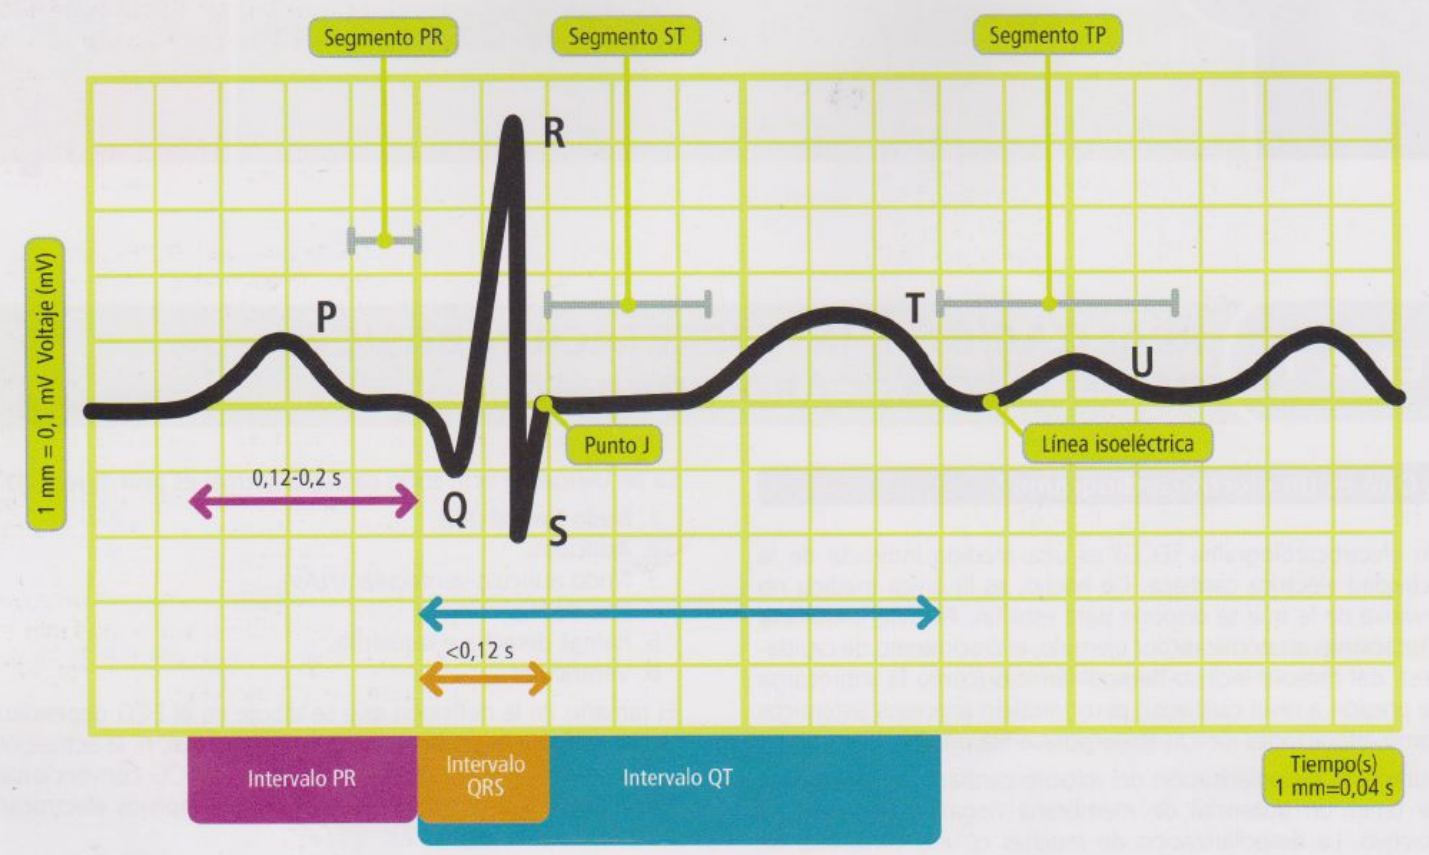
\includegraphics[scale=0.25]{images/teoria_ecg.png}
\end{center}
\caption{Senyal teòrica d'un ECG i els seus segments}
\label{fig: ecg_arduino}
\end{figure}
%
\noindent Hi ha molta literatura que permet identificar malalties analitzant els diferents segments, la seva durada i l'amplitud de la senyal. Tot i que considerem que es podria programar un algorisme per fer un anàlisi de la senyal, ens hem centrat en calcular la freqüència cardíaca amb la fórmula de l'equació \ref{bpm}.
\begin{equation} \label{bpm}
\beta= \frac{1}{T}*1000*60
\end{equation}

\noindent $\beta$: freqüència cardíaca (bpm).\\
$T$: període entre pic i pic (ms).


\section{Rang de freqüència cardíaca habitual}
Una persona al llarg de la seva vida sol tenir una freqüència cardíaca en repòs variable. La medicina no és una ciència exacte i per tant no és d'estranyar que cada autor o referència doni uns nivells habituals de freqüència cardíaca lleugerament diferents.\\
\newline Per donar una referència, la majoria de la població té una freqüència cardíaca que es troba dins l'interval donat a la Taula \ref{tab:consums}:
\begin{table}[H]
\small
  \centering
    \begin{tabu} to \textwidth {|X[4]|X|X|} \hline
     & \multicolumn{2}{|c|}{Freqüència cardíaca (bpm)} \\
    \hline
    \multicolumn{1}{|l}{Edat} & \multicolumn{1}{|l}{Mínim} & \multicolumn{1}{|l|}{Màxim} \\ \hline \hline
    Recent nascuts, de 0 a 1 mes & 70 & 190 \\ \hline
    Bebès de 1 a 11 mesos d'edat & 80 & 160 \\ \hline
    Nens de 1 a 2 anys d'edat  & 80 & 130 \\ \hline
    Nens de 3 a 4 anys d'edat & 80 & 120  \\ \hline
    Nens de 5 a 9 anys d'edat  & 75 & 115 \\ \hline
    Nens a partir de 10 anys i persones adultes & 50 & 100 \\ \hline
    Esportistes amb bon entrenament cardiovascular & 40 & 60 \\ \hline

    \end{tabu}%
  \label{tab:addlabel}%
    \caption{Freqüències cardíaques habituals segons l'edat}
    \label{tab:consums}
\end{table}%

\noindent Com veiem, el rang de freqüència cardíaca és molt gran, especialment durant l'edat adulta. No es pot dir que una persona tingui una malaltia important per tenir el cor a 80 bpm, per exemple. Creiem més important conèixer l'evolució de la freqüència cardíaca d'una persona al llarg de la seva vida que no pas conèixer aquesta magnitud en un instant determinat.\\
\newline És evident que tenir una freqüència cardíaca de 0 bpm o similar indica, sens dubte, que la persona ha patit una parada cardíaca.\\
\newline Es diu que la freqüència cardíaca màxima d'una persona segons la seva edat ve regida per l'equació \ref{beta}.
\begin{equation} \label{beta}
\beta_{opt}=220 - e
\end{equation}

\noindent $e$: edat de la persona (anys).\\

%
%
%
%
%


\section{Electrocardiògrafs actuals i solució proposada}
Tradicionalment un electrocardiograma es podia fer amb un electrocardiògraf analògic, el qual pot ser tant simple com un amplificador diferencial que dona la diferència de tensió entre dos elèctrodes i l'amplifica. La referència d'aquesta tensió pot ser el nivell de tensió d'un tercer elèctrode, el qual actua com a massa.\\
\newline Aquesta configuració de 3 elèctrodes és la que nosaltres escollim, per bé que n'hi ha d'altres de viables que funcionen amb més elèctrodes i que poden ser més fiables.
\begin{figure}[H]
\begin{center}
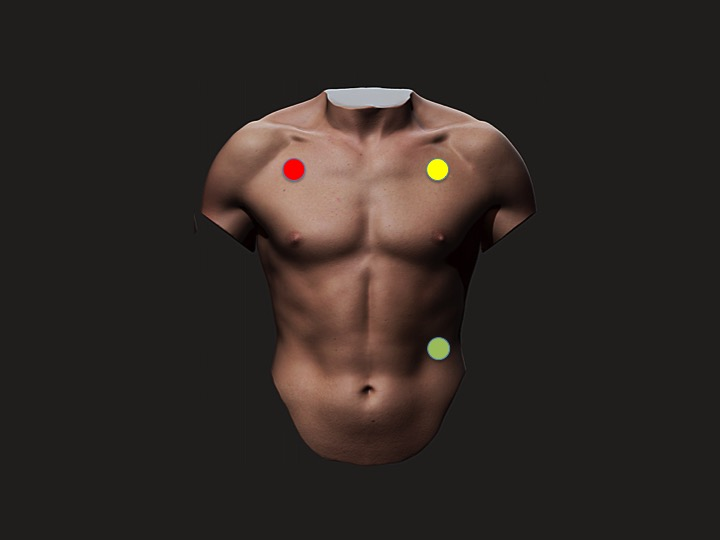
\includegraphics[scale=0.5]{images/electrodos.jpg}
\end{center}
\caption{Col·locació de 3 elèctrodes}
\label{fig: electrodes}
\end{figure}
%ampliar aquí.
%
%
\noindent Un electrocardiògraf analògic no enregistra dades de freqüència cardíaca. Si es desplaça un tros de paper de forma constant i la senyal analògica de tensió s'amplifica adequadament i s'aconsegueix desplaçar de forma proporcional a la tensió llegida una agulla, la qual té un bolígraf o similar a un dels seus extrems amb què pot dibuixar un electrocardiograma.
\begin{figure}[H]
\begin{center}
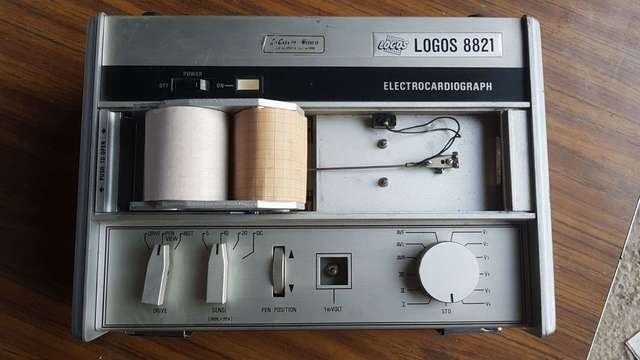
\includegraphics[scale=0.5]{images/ecg.jpg}
\end{center}
\caption{Electrocardiògraf analògic}
\label{fig: electrodes}
\end{figure}
\noindent L'electrònica digital permet estalviar-se dibuixar la senyal de forma analògica sobre un paper. Es basa en mostrejar a alta velocitat la senyal analògica d'entrada i enregistrar les dades. D'aquesta manera es poden representar les dades captades en un pla, donant lloc a l'electrocardiograma.
\begin{figure}[H]
\begin{center}
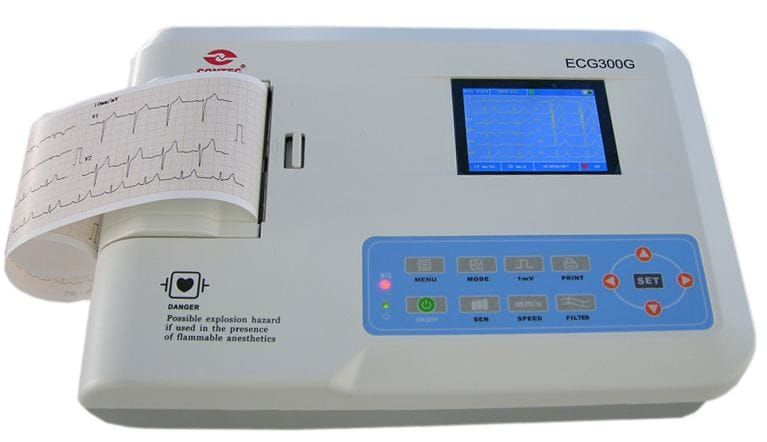
\includegraphics[scale=0.35]{images/ecg_2.jpg}
\end{center}
\caption{Electrocardiògraf actual}
\label{fig: electrodes}
\end{figure}
\noindent Els electrocardiògrafs digitals tenen l'avantatge de poder enregistrar dades, o sigui, tenen memòria. Els electrocardiògrafs analògics no ofereixen aquesta possibilitat. Tot i això, l'equip de la imatge, per exemple, tot i ser digital, funciona com un electrocardiògraf analògic en el sentit de què només imprimeix, no tracta ni emmagatzema de cap manera les dades.\\
\newline Al llarg del treball es mostra com no només es dissenya un electrocardiògraf digital, sinó que aquest guarda dades que són consultables mitjançant una interfície clara, cosa que molts no electrocardiògrafs comercials no fan.\\
\newline Tot i això, també donem l'opció a visualitzar l'electrocardiograma a través del por sèrie de l'Arduino Nano. Mostregem a una freqüència suficient, la qual assegura que no ens perdem cap pic ni cap dada significativa de l'electrocardiograma.
\begin{figure}[H]
\begin{center}
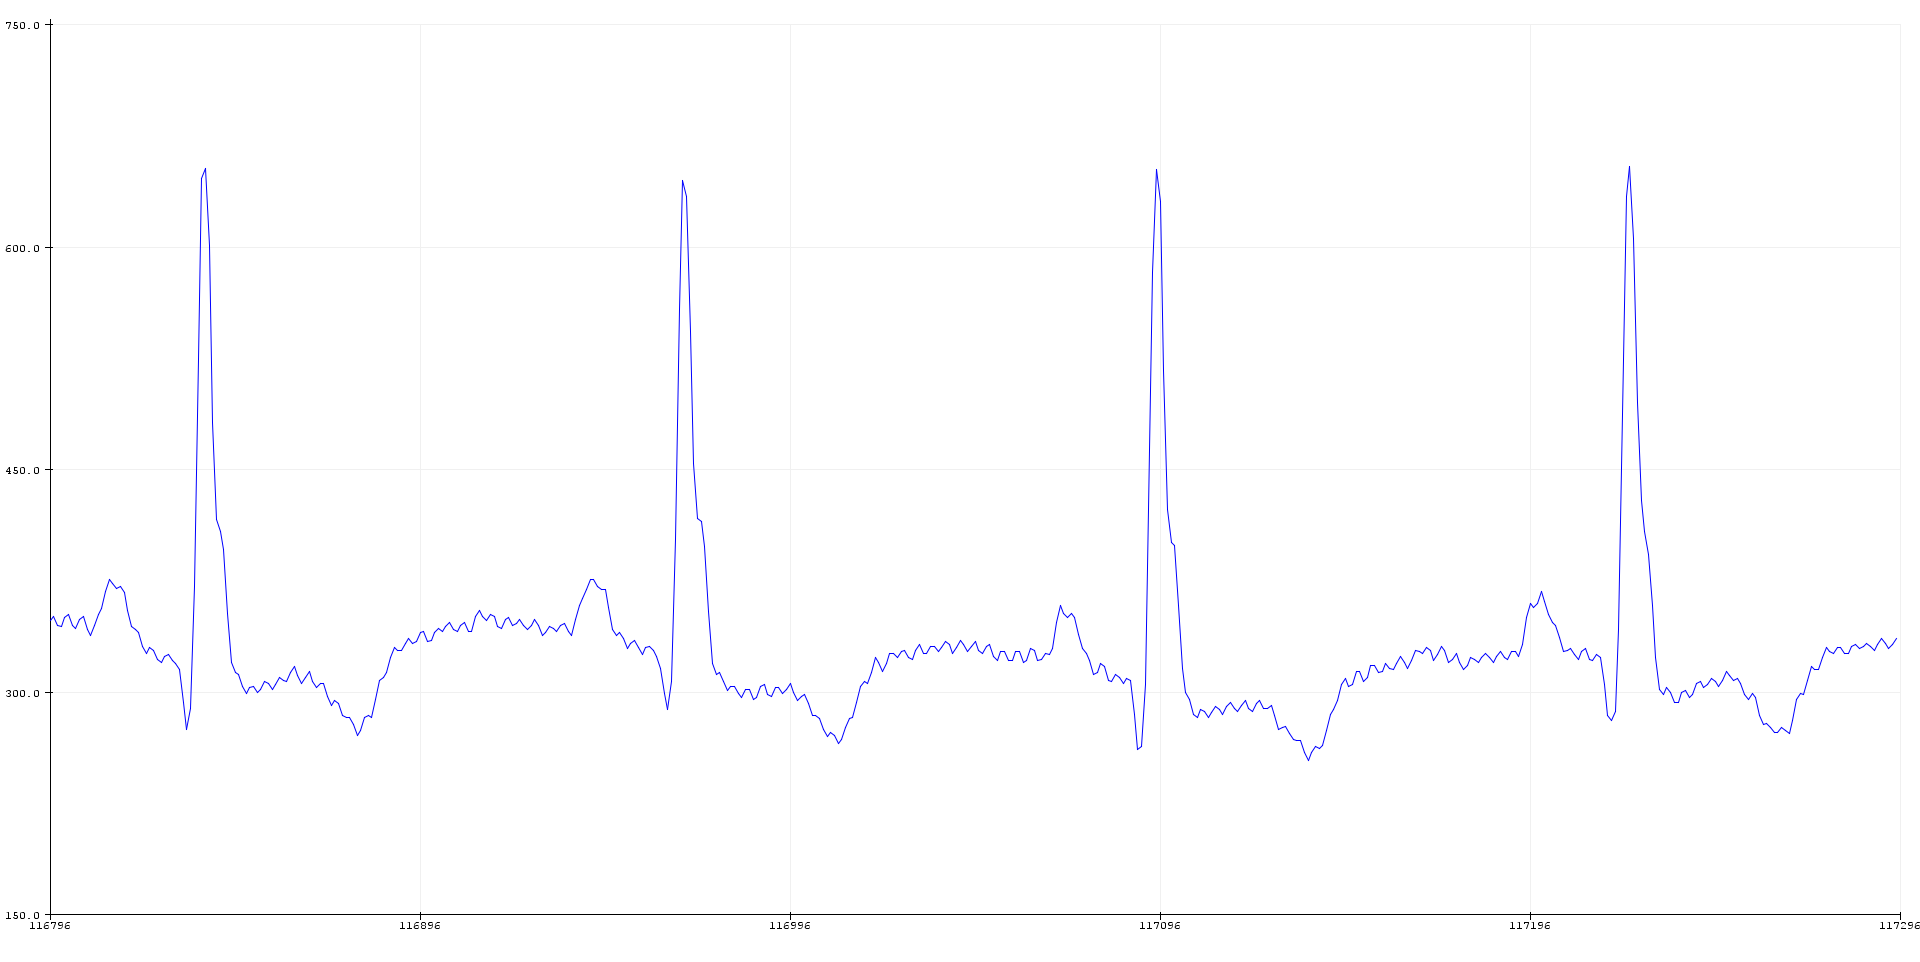
\includegraphics[scale=0.25]{images/ecg_arduino.png}
\end{center}
\caption{Electrocardiògraf donat per l'Arduino}
\label{fig: ecg_arduino}
\end{figure}
%

%




